% meta.concepts: 2D rigid-body force equilibrium
% meta.tags: realistic
% acknowledge: Peter Seiler & Luke Melander graciously shared Spring 2019 course material
% source: 2019 P. Seiler AEM2011 HW 5

A large rocket is assembled and taken to the launch pad in a horizontal orientation. To prepare it for launch,
it must be hoisted into a vertical position at the launch tower using an electric winch. The initial geometry is
shown in the left diagram below. The rocket has a bracket at its base which is connected to the ground via
a frictionless pin at the origin $O$. The cable first contacts the winch spool at point $B$ located at $(L/10){\bf i} + L{\bf j}$
(assume B does not move as $\theta$ changes). The cable from the winch is connected to the rocket's center of gravity,
located initially (when $\theta = 0^\circ$) at $-L{\bf i}$. Assume that the hoisting action begins instantaneously and is carried
out at a constant speed (such that both the net force and net moment acting on the rocket are always zero).
The geometry after the rocket has been hoisted to an angle $\theta$ is shown in the right diagram below.
\begin{enumerate}
  \item If the rocket weighs 20,000 lbs and $L = 24 ft$, find the tension in the cable and the reaction at the origin when $\theta = 40^\circ$.
  \item For what value of $\theta$ is the tension in the cable $T$ the highest? Also compute the maximum tension $T_{max}$.
  \item You are the engineer in charge of sizing the parts for the winch. You may choose from a selection of three motors two spools:
  \begin{itemize}
	\item Motor A costs \$4,000 and has a maximum torque of 25,000 lb-ft
	\item Motor B costs \$5,000 and has a maximum torque of 35,000 lb-ft
	\item Motor C costs \$6,000 and has a maximum torque of 50,000 lb-ft
        \item Spool X costs \$1,000 and has a diameter of 2 ft
	\item Spool Y costs \$2,000 and has a diameter of 3 ft
  \end{itemize}
Find the cheapest viable combination of motor and spool for the winch.
\end{enumerate}

\begin{figure}[ht!]
  \centering
  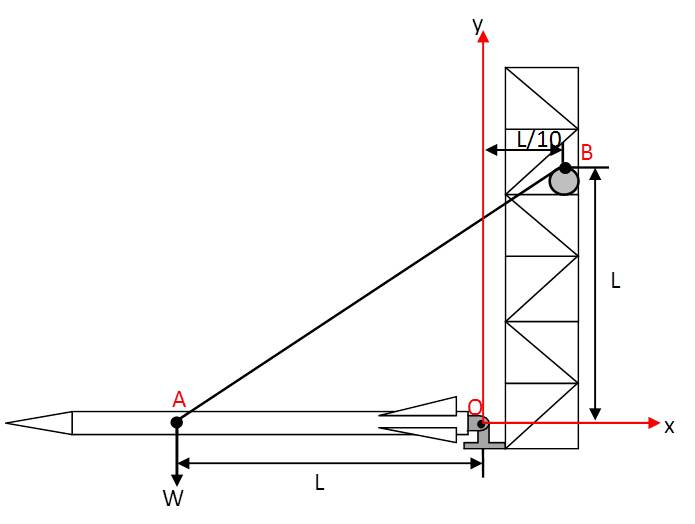
\includegraphics[height=1.8in]{figa.png}
  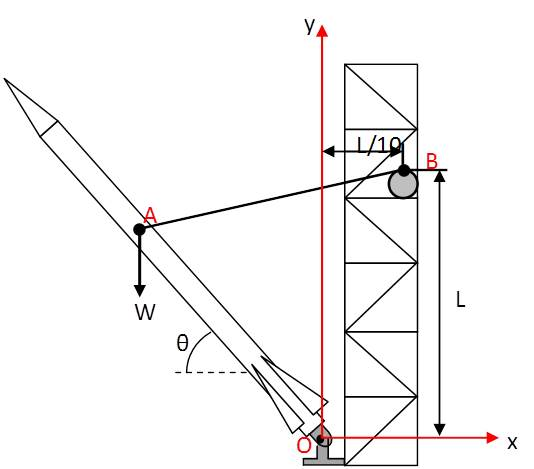
\includegraphics[height=1.8in]{figb.png}
\end{figure}

\iftoggle{flagSoln}{%
\vspace{.5cm}
\rule{\textwidth}{.4pt}
\vspace{.5cm}
\textbf{Solution:}
\begin{figure}[ht!]
  \centering
  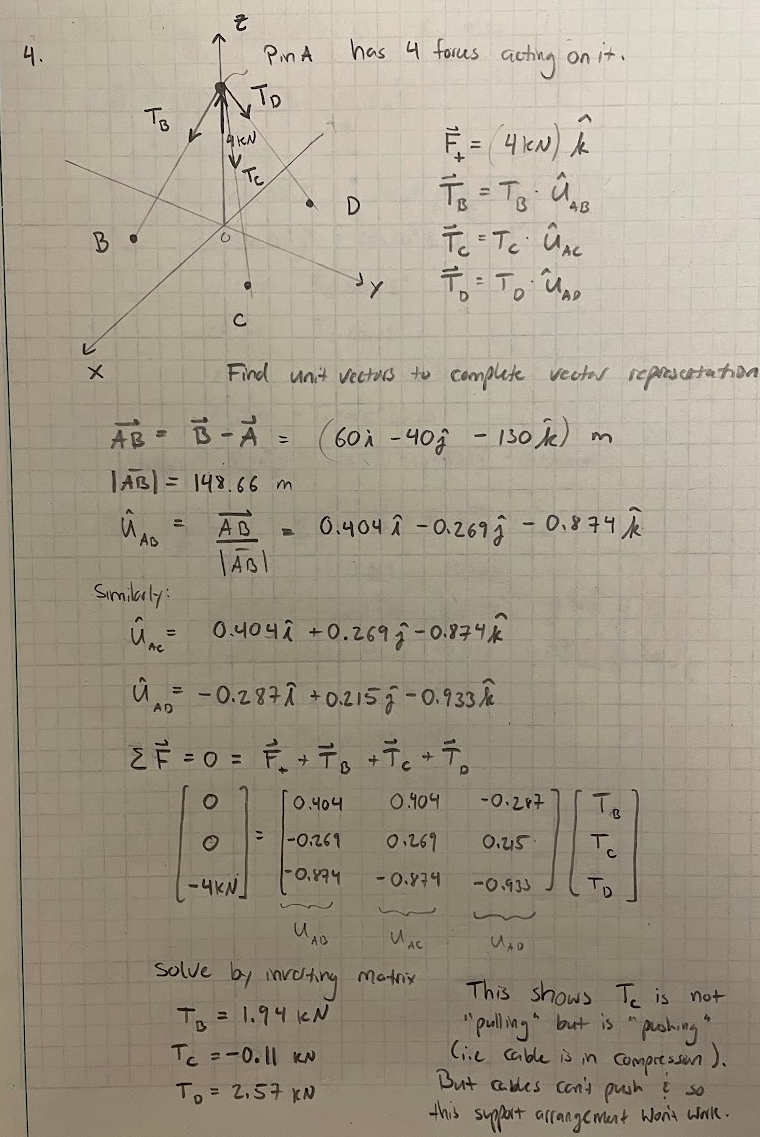
\includegraphics[width=0.9\textwidth,
	           height=0.3\textheight,
		   keepaspectratio]{soln.png}
\end{figure}
}{%
}%
